\documentclass[12pt]{article}
\usepackage[utf8]{inputenc}

\usepackage{lmodern}

\usepackage{enumitem}
\usepackage[margin=2cm]{geometry}

\usepackage{amsmath, amsfonts, amssymb}
\usepackage{graphicx}
\usepackage{subfigure}
\usepackage{tikz}
\usepackage{pgfplots}
\usepackage{multicol}

\usepackage{titlesec}
\usepackage{environ}
\usepackage{xcolor}
\usepackage{fancyhdr}
\usepackage[colorlinks = true, linkcolor = black]{hyperref}
\usepackage{xparse}
\usepackage{enumitem}
\usepackage{comment}
\usepackage{wrapfig}
\usepackage[capitalise]{cleveref}
\usepackage{epsdice}
\usepackage{circledsteps}

\usepackage{url}
\usepackage{calc}
%\usepackage{subcaption}
\usepackage[indent=0pt]{parskip}

\usepackage{array}
\usepackage{blkarray,booktabs, bigstrut}
\usepackage{bigints}

\pgfplotsset{compat=1.16}

% MATH commands
\newcommand{\ga}{\left\langle}
\newcommand{\da}{\right\rangle}
\newcommand{\oa}{\left\lbrace}
\newcommand{\fa}{\right\rbrace}
\newcommand{\oc}{\left[}
\newcommand{\fc}{\right]}
\newcommand{\op}{\left(}
\newcommand{\fp}{\right)}

\newcommand{\bi}{\mathbf{i}}
\newcommand{\bj}{\mathbf{j}}
\newcommand{\bk}{\mathbf{k}}
\newcommand{\bF}{\mathbf{F}}

\newcommand{\mR}{\mathbb{R}}
\newcommand{\mC}{\mathbb{C}}
\newcommand{\mT}{\mathbb{T}}
\newcommand{\mD}{\mathbb{D}}

\newcommand{\ra}{\rightarrow}
\newcommand{\Ra}{\Rightarrow}

\newcommand{\sech}{\mathrm{sech}\,}
\newcommand{\csch}{\mathrm{csch}\,}
\newcommand{\curl}{\mathrm{curl}\,}
\newcommand{\dive}{\mathrm{div}\,}

\newcommand{\ve}{\varepsilon}
\newcommand{\spc}{\vspace*{0.5cm}}

\DeclareMathOperator{\Ran}{Ran}
\DeclareMathOperator{\Dom}{Dom}
\DeclareMathOperator{\re}{Re}
\DeclareMathOperator{\im}{Im}
%\DeclareMathOperator{\arg}{arg}

\usepackage{pifont}

\newcommand{\club}{\ding{168}}
\newcommand{\spade}{\ding{171}}
\newcommand{\ddiamond}{{\color{red}\ding{169}}}
\newcommand{\heart}{{\color{red}\ding{170}}}

% Playing card
\newcommand{\cardH}[2]{%
\begin{tikzpicture}[trim right = #2pt, scale=0.1]
  % Card outline
  \draw[thick, red] (0,0) rectangle (5,3.5);
  % Card suit and value
  \node at (1.4,1.75) {\tiny\color{red} #1};
  \node[red] at (3.5, 1.75) {\scriptsize\heart};
\end{tikzpicture}
}
\newcommand{\cardD}[2]{%
\begin{tikzpicture}[trim right = #2pt, scale=0.1]
  % Card outline
  \draw[thick, red] (0,0) rectangle (5,3.5);
  % Card suit and value
  \node at (1,1.75) {\tiny\color{red} #1};
  \node[red] at (3.5, 1.75) {\footnotesize\ddiamond};
\end{tikzpicture}
}
\newcommand{\cardS}[2]{%
\begin{tikzpicture}[trim right = #2pt, scale=0.1]
  % Card outline
  \draw[thick, black] (0,0) rectangle (5,3.5);
  % Card suit and value
  \node at (1,1.75) {\tiny\color{black} #1};
  \node[black] at (3.5, 1.75) {\footnotesize\spade};
\end{tikzpicture}
}
\newcommand{\cardC}[2]{%
\begin{tikzpicture}[trim right = #2pt, scale=0.1]
  % Card outline
  \draw[thick, black] (0,0) rectangle (5,3.5);
  % Card suit and value
  \node at (1,1.75) {\tiny\color{black} #1};
  \node[black] at (3.5, 1.75) {\footnotesize\club};
\end{tikzpicture}
}

%% Defining example environment
\newcounter{totNumProblems}
\newcounter{problem}[section]
\NewEnviron{problem}%
	{%
	\noindent\refstepcounter{problem}\refstepcounter{totNumProblems}\fcolorbox{gray!40}{gray!40}{\textsc{\textcolor{black}{Problem~\theproblem.}}}%
	%\fcolorbox{black}{white}%
		{  %\parbox{0.95\textwidth}%
			{
			\BODY
			}%
		}%
	}


%% Redefining sections
\newcommand{\sectionformat}[1]{%
    \begin{tikzpicture}[baseline=(title.base)]
        \node[rectangle, draw] (title) {#1 \thesection};
    \end{tikzpicture}
    
    \noindent\hrulefill
}

\renewcommand{\thesection}{\Alph{section}}
\renewcommand{\thesubsection}{\Alph{section}.\arabic{subsection}}

% default values copied from titlesec documentation page 23
% parameters of \titleformat command are explained on page 4
\titleformat{\section}{\centering\normalfont\large\scshape}{}{1em}{\centering\sectionformat}

%% Set counters for sections to none
%\setcounter{secnumdepth}{0}

%% Set the footer/headers
\pagestyle{fancy}
\fancyhf{}
\renewcommand{\headrulewidth}{0pt}
\renewcommand{\footrulewidth}{2pt}
\lfoot{P.-O. Paris{\'e}}
\cfoot{MATH 471}
\rfoot{Page \thepage}

\begin{document}
\hrulefill

\begin{minipage}{0.33\textwidth}
\textsc{Math 471}
\end{minipage} \hfill 
\begin{minipage}{0.32\textwidth}
\centering
\textsc{Solutions to Problems} \\
Chapter E
\end{minipage}
 \hfill 
 \begin{minipage}{0.33\textwidth}
 \flushright \textsc{Fall 2023}
 \end{minipage}

\hrulefill

\setcounter{section}{5}

\subsection{Bivariate Distributions}

\begin{problem}
See Example E.3c).
\end{problem}

\subsection{Continuous Random Vectors}

\begin{problem}
Let $R = [a, b] \times [c, d]$. Then, we have
    \[
        P (a \leq X \leq b , c \leq Y \leq d ) = \iint_R f_{X, Y} (x, y) \, dA = \int_c^d \int_a^b f_{X, Y} (x, y) \, dx dy
    \]
Notice that, for any positive integer $n$,
    \[
        P (X = a , c \leq Y \leq d ) = \lim_{n \ra \infty} P (a \leq X \leq a + \frac{1}{n}, c \leq Y \leq d )
    \]
by the continuity of probability measure. Therefore, 
    \[
        P (X = a , c \leq Y \leq d ) = \lim_{n \ra \infty} \int_c^d \int_a^{a + \frac{1}{n}} f_{X, Y} (x, y) \, dx dy = \int_c^d \int_a^a f_{X, Y} (x, y) \, dx dy = 0 .
    \]
By performing similar calculations, we have $P (a \leq X \leq b , Y = c ) = 0$. 

Now, we have    
    \[
        R = (\{ a \} \times [c, d] ) \cup ( \{ b \} \times [c, d] ) \cup ( [a, b] \times \{ c \} ) \cup ([a, b] \times \{ d \} ) \cup \big( (a, b) \times (c, d) \big)
    \]
and therefore
    \begin{align*}
        P (a \leq X \leq b , c \leq Y \leq d ) &= P (X = a , c \leq Y \leq d ) + P (X = b , c \leq Y \leq d )  \\ 
        & \quad + P (a \leq X \leq b , Y = c) + P (a \leq X \leq b , Y = d ) \\ 
        & \quad + P (a < X < b , c < Y < d ) \\ 
        &= 0 + 0 + 0 + 0 + P (a < X < b , c < Y < d ) \\ 
        &= P (a < X < b , c < Y < d ) . \tag*{$\square$}
    \end{align*}
\end{problem}

\begin{problem}
\begin{enumerate}[label=\alph*)]
\item We must have
    \[
        \int_{-\infty}^\infty \int_{-\infty}^\infty f_{X, Y} (x, y) \, dx dy = 1 .
    \]
Therefore, replacing $f_{X, Y}$ by its expression, we find that it must satisfies
    \[
        \int_0^1 \int_0^1 k xy \, dx dy = 1 \quad \iff \quad \frac{k}{4} = 1 \quad \iff \quad k = 4 .
    \]
\item If $x < 0$, then $F_{X, Y} (x, y) = 0$. If $y < 0$, then $F_{X, Y} (x, y) = 0$ because $f_{X, Y} (x, y)= 0$ there. 

So, assume that $x \geq 0$ and $y \geq 0$. There are four cases to consider.
    \begin{enumerate}[label=\arabic*.]
        \item Assume $0 \leq x \leq 1$ and $0 \leq y \leq 1$. In that case, we get
            \[
                F_{X, Y} (x, y) = \int_0^y \int_0^x 4 uv \, du dv = x^2 y^2 .
            \]
        \item Assume $0 \leq x \leq 1$ and $y > 1$. In that case, we get
            \[
                F_{X, Y} (x, y) = \int_0^1 \int_0^x 4 uv \, du dv = x^2 .
            \]
        \item Assume $x > 1$ and $0 \leq y \leq 1$. In that case, we get
            \[
                F_{X, Y} (x, y) = \int_0^y \int_0^1 4uv \, du dv = y^2 .
            \]
        \item Assume $x > 1$ and $y > 1$. In that case, we get
            \[
                F_{X, Y} (x, y) = \int_0^1 \int_0^1 4uv \, du dv = 1 .
            \]
    \end{enumerate}
Hence, the joint distribution of $X$ and $Y$ is
    \[
        F_{X, Y} (x, y) = \left\lbrace \begin{matrix} x^2 y^2 & 0 \leq x \leq 1 , 0 \leq y \leq 1 \\ 
        x^2 & 0 \leq x \leq 1 , y > 1 \\ 
        y^2 & x > 1 , 0 \leq y \leq 1 \\ 
        1 & x > 1 , y > 1 \\ 
        0 & \text{elsewhere.} \end{matrix} \right. 
    \]
\item Find $P (X \leq 0.5 , Y \leq 0.75)$. Since $(0.5, 0.75) \in [0, 1] \times [0, 1]$, we obtain from (b),
    \[
        P (X \leq 0.5 , Y \leq 0.75) = F_{X, Y} (0. 5, 0.75) = (0.5)^2 (0.75)^2 = \frac{9}{64} . \tag*{$\square$}
    \]
\end{enumerate}
\end{problem}

\begin{problem}
We have $\{ X \leq Y \} = \{ (X, Y) \, : \, X \leq Y \}$. Let $R = \{ (x, y) \, : \, x \leq y \}$. Therefore,
    \[
        P (X \leq Y ) = P ( (X, Y) \in R ) = \iint_R f_{X, Y} (x, y) \, dA = \iint_{D \cap R} \frac{1}{\pi} \, dA = \frac{\mathrm{Area} (D \cap R )}{\pi} .
    \]
Notice that $D \cap R = \{ (r, \theta ) \, : \, 0 \leq r \leq 1 , \pi/4 \leq \theta \leq 5 \pi / 4 \}$ and this is half of the region inside a circle of radius $1$. Hence
    \[
        P (X \leq Y ) = \frac{\frac{\pi}{2}}{\pi} = \frac{1}{2} . \tag*{$\square$}
    \]

\end{problem}

\subsection{Marginals and Independence}

\begin{problem}
    \begin{enumerate}[label=\alph*)]
        \item The distribution function of $X$ is given by $F_X (x) = \lim_{y \ra \infty} F_{X, Y} (x, y)$. Using the fact that $X, Y$ jointly continuous, we get
            \[
                F_X (x) = \int_{-\infty}^x \int_{-\infty}^\infty f_{X, Y} (u, y ) \, dy du .
            \]
        Taking the derivative, we get
            \[
                f_X (X) = \int_{-\infty}^\infty f_{X, Y} (x, y) \, dy .
            \]
        \item The distribution function of $Y$ is given by $F_Y (y) = \lim_{x \ra \infty} F_{X, Y} (x, y)$. Using the fact again that $X, Y$ are jointly continuous, we get
            \[
                F_Y (y) = \int_{-\infty}^y \int_{-\infty}^\infty f_{X, Y} (x, v ) \, dx dv .
            \]
        Taking the derivative, we get
            \[
                f_Y (y) = \int_{-\infty}^\infty f_{X, Y} (x, y) \, dx . \tag*{$\square$}
            \]
    \end{enumerate}
\end{problem}


\begin{problem}
    \begin{enumerate}[label=\alph*)]
        \item Below is a sketch of the density function using Desmos.
            \begin{center}
            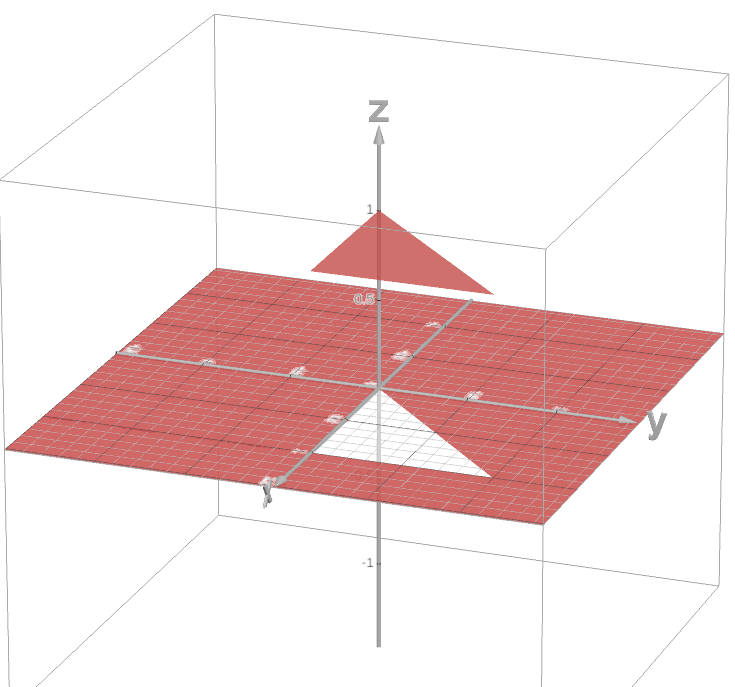
\includegraphics[scale=0.3]{figure1.png}
            \end{center}
        \item After some calculations, we get
            \[
                f_X (x) = \left\lbrace \begin{matrix} x & 0 \leq x \leq 1 \\ 0 & \text{elsewhere.} \end{matrix} \right.
            \]
        and
            \[
                f_Y (y) = \left\lbrace \begin{matrix} 1 - y & 0 \leq y \leq 1 \\ 0 & \text{elsewhere.} \end{matrix} \right. 
            \]
        We see that $f_{X, Y} (x, y) \neq f_X (x) f_Y (y)$ and therefore $X$ and $Y$ are dependent. \hfill $\square$
    \end{enumerate}
\end{problem}

\begin{problem}
    \begin{enumerate}[label=\alph*)]
        \item Below is a sketch of the density function using Desmos.
            \begin{center}
            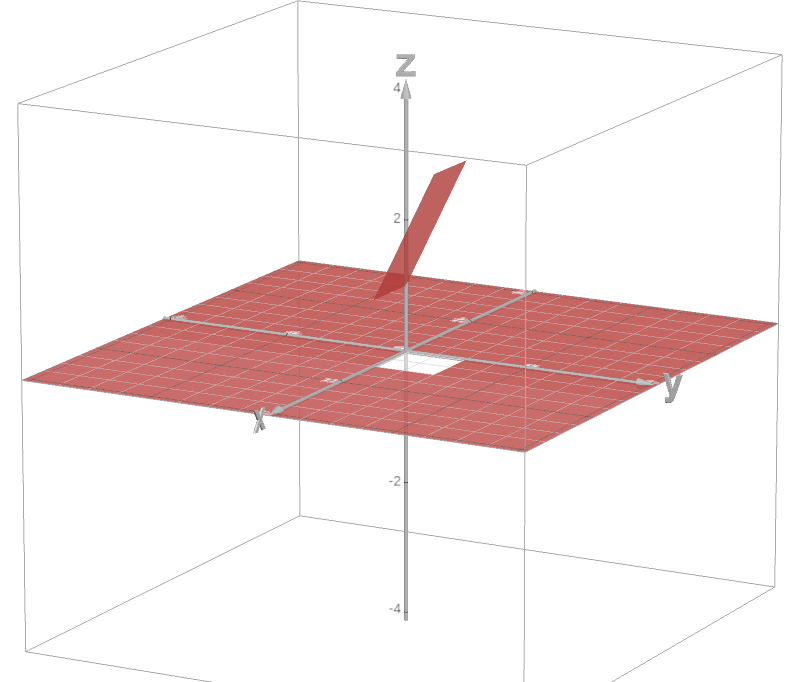
\includegraphics[scale=0.3]{figure2.png}
            \end{center}
        \item After some calculations, we get
            \[
                f_X (x) = \left\lbrace \begin{matrix} 1 & 0 \leq x \leq 1 \\ 0 & \text{elsewhere.} \end{matrix} \right.
            \]
        and
            \[
                f_Y (y) = \left\lbrace \begin{matrix} y + 1/2 & 0 \leq y \leq 1 \\ 0 & \text{elsewhere.} \end{matrix} \right. 
            \]
        We see that $f_{X, Y} (x, y) = f_X (x) f_Y (y)$ and therefore $X$ and $Y$ are independent. \hfill $\square$
    \end{enumerate}
\end{problem}

\begin{problem}
Let $X$ be the time of arrival of the passenger and let $Y$ be the time of arrival of the bus. We have $0 \leq X \leq 60$ and $0 \leq Y \leq 60$. Also, $X , Y \sim U (0, 60)$. Since there are independent, their joint density function is 
    \[
        f_{X, Y} (x, y) = f_X (x) f_Y (y) = \left\lbrace \begin{matrix} \frac{1}{3600} & (x, y) \in [0, 1] \times [0, 1] \\ 0 & \text{elsewhere} . \end{matrix} \right. 
    \]
Let $a$ be the arrival time of the passenger at the bus station. Since the passenger waits 15min for a bus to arrive, the bus must stops at the bus station between $a$min and $(a + 15)$min. Therefore, the probability is
    \[
        P (a \leq X \leq a + 15 , a \leq Y \leq a + 15 ) = \frac{15 \cdot 15}{3600} = \frac{25}{400} = \frac{1}{16} = 0.0625 . \tag*{$\square$}
    \]
\end{problem}

%\subsection{Sums of Random Variables}

\subsection{Important Measurements}

\begin{problem}
Since $X$ and $Y$ are independent, then
    \[
        \mathrm{Cov} (X, Y) = \mathrm{Exp} (X Y) - \mathrm{Exp} (X) \mathrm{Exp} (Y) = 0
    \]
because $\mathrm{Exp} (XY) = \mathrm{Exp} (X) \mathrm{Exp} (Y)$.
\end{problem}

\begin{problem}
In this case, we need the Cauchy Schwarz inequality:
    \[
        |\mathrm{Exp} (XY)| \leq \sqrt{\mathrm{Exp} (X^2)} \sqrt{\mathrm{Exp} (Y^2)} .
    \]
Using that, we see that
    \[
        |\mathrm{Cov} (X, Y)| = \mathrm{Exp} ( (X - \mu_X ) (Y- \mu_Y)) \leq \sqrt{\mathrm{Exp} ( (X-\mu_X)^2)} \sqrt{\mathrm{Exp} ( (Y - \mu_Y)^2)} = \sigma_X \sigma_Y .
    \]
Therefore,
    \[
        |\rho (X, Y) | = \left| \frac{\mathrm{Cov} (X, Y)}{\sigma_X \sigma_Y} \right| \leq 1 . \tag*{$\square$}.
    \]
\end{problem}

\begin{problem}
    \begin{enumerate}[label=\alph*)]
        \item By definition,
            \[
                \mathrm{Cov} (X, Y) = \mathrm{Exp} ( (X -\mu_X) (Y - \mu_Y)) = \mathrm{Exp} ( (Y- \mu_Y) (X - \mu_X )) = \mathrm{Cov} (Y, X) .
            \]
        \item By the formula of the variance,
            \begin{align*}
                \mathrm{Var} (aX + bY) &= \mathrm{Exp} ( (aX + bY)^2)) - (\mathrm{Exp} (aX + bY))^2 \\ 
                &= a^2 \mathrm{Exp} (X^2) + 2ab \mathrm{Exp} (XY) + b^2 \mathrm{Exp} (Y^2) - a^2\mu_X^2 - 2ab \mu_X \mu_Y - b^2 \mu_Y^2 \\ 
                &= a^2 (\mathrm{Exp} (X^2) - \mu_X^2) + b^2 (\mathrm{Exp} (Y^2) - \mu_Y^2) + 2ab (\mathrm{Exp} (XY) - \mu_X \mu_Y ) \\ 
                &= a^2 \mathrm{Var} (X) + b^2 \mathrm{Var} (Y) + 2ab \mathrm{Cov} (X, Y) . 
            \end{align*} 
        \item By definition,
            \[
                \mathrm{Cov} (X, X) = \mathrm{Exp} ( (X - \mu_X) (X - \mu_X )) = \mathrm{Var} (X) . \tag*{$\square$}
            \]
    \end{enumerate}
\end{problem}

\begin{problem}
    \begin{enumerate}[label=\alph*)]
            \item Since $\mathrm{Cov} (X, X) = \mathrm{Var} (X)$, we find that $\mathrm{Cov} (X, X) = 2$. 
            \item Since $\rho (X, Y) \in [-1, 1]$, we see that
                \[
                    \frac{\mathrm{Cov} (X, Y)}{\sigma_X \sigma_Y} \leq 1 \quad \Rightarrow \quad \mathrm{Cov} (X, Y) \leq (\sqrt{2}) (2\sqrt{2}) = 4 . \tag*{$\square$}
                \]
    \end{enumerate}
\end{problem}

\end{document}